
% The first stasheff identity for DG-morphisms using trees



\begin{center}
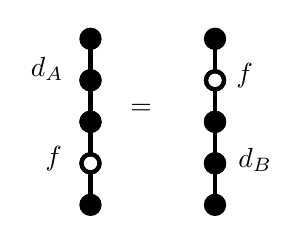
\begin{tikzpicture}[x=0.75pt,y=0.75pt,yscale=-1,xscale=1]
%uncomment if require: \path (0,513); %set diagram left start at 0, and has height of 513

%Straight Lines [id:da9149295825374517] 
\draw [line width=1.5]    (50,120) -- (50,103.36) ;
\draw [shift={(50,100)}, rotate = 270] [color={rgb, 255:red, 0; green, 0; blue, 0 }  ][line width=1.5]      (0, 0) circle [x radius= 4.36, y radius= 4.36]   ;
\draw [shift={(50,120)}, rotate = 270] [color={rgb, 255:red, 0; green, 0; blue, 0 }  ][fill={rgb, 255:red, 0; green, 0; blue, 0 }  ][line width=1.5]      (0, 0) circle [x radius= 4.36, y radius= 4.36]   ;
%Straight Lines [id:da6451654153315307] 
\draw [line width=1.5]    (50,96.65) -- (50,80) ;
\draw [shift={(50,80)}, rotate = 270] [color={rgb, 255:red, 0; green, 0; blue, 0 }  ][fill={rgb, 255:red, 0; green, 0; blue, 0 }  ][line width=1.5]      (0, 0) circle [x radius= 4.36, y radius= 4.36]   ;
\draw [shift={(50,100)}, rotate = 270] [color={rgb, 255:red, 0; green, 0; blue, 0 }  ][line width=1.5]      (0, 0) circle [x radius= 4.36, y radius= 4.36]   ;
%Straight Lines [id:da951655139734809] 
\draw [line width=1.5]    (110,80) -- (110,63.36) ;
\draw [shift={(110,60)}, rotate = 270] [color={rgb, 255:red, 0; green, 0; blue, 0 }  ][line width=1.5]      (0, 0) circle [x radius= 4.36, y radius= 4.36]   ;
\draw [shift={(110,80)}, rotate = 270] [color={rgb, 255:red, 0; green, 0; blue, 0 }  ][fill={rgb, 255:red, 0; green, 0; blue, 0 }  ][line width=1.5]      (0, 0) circle [x radius= 4.36, y radius= 4.36]   ;
%Straight Lines [id:da5333607615257305] 
\draw [line width=1.5]    (110,56.65) -- (110,40) ;
\draw [shift={(110,40)}, rotate = 270] [color={rgb, 255:red, 0; green, 0; blue, 0 }  ][fill={rgb, 255:red, 0; green, 0; blue, 0 }  ][line width=1.5]      (0, 0) circle [x radius= 4.36, y radius= 4.36]   ;
\draw [shift={(110,60)}, rotate = 270] [color={rgb, 255:red, 0; green, 0; blue, 0 }  ][line width=1.5]      (0, 0) circle [x radius= 4.36, y radius= 4.36]   ;
%Straight Lines [id:da3030831638766034] 
\draw [line width=1.5]    (110,100) -- (110,80) ;
\draw [shift={(110,80)}, rotate = 270] [color={rgb, 255:red, 0; green, 0; blue, 0 }  ][fill={rgb, 255:red, 0; green, 0; blue, 0 }  ][line width=1.5]      (0, 0) circle [x radius= 4.36, y radius= 4.36]   ;
\draw [shift={(110,100)}, rotate = 270] [color={rgb, 255:red, 0; green, 0; blue, 0 }  ][fill={rgb, 255:red, 0; green, 0; blue, 0 }  ][line width=1.5]      (0, 0) circle [x radius= 4.36, y radius= 4.36]   ;
%Straight Lines [id:da32521299307207774] 
\draw [line width=1.5]    (110,120) -- (110,100) ;
\draw [shift={(110,100)}, rotate = 270] [color={rgb, 255:red, 0; green, 0; blue, 0 }  ][fill={rgb, 255:red, 0; green, 0; blue, 0 }  ][line width=1.5]      (0, 0) circle [x radius= 4.36, y radius= 4.36]   ;
\draw [shift={(110,120)}, rotate = 270] [color={rgb, 255:red, 0; green, 0; blue, 0 }  ][fill={rgb, 255:red, 0; green, 0; blue, 0 }  ][line width=1.5]      (0, 0) circle [x radius= 4.36, y radius= 4.36]   ;
%Straight Lines [id:da02196000233385731] 
\draw [line width=1.5]    (50,80) -- (50,60) ;
\draw [shift={(50,60)}, rotate = 270] [color={rgb, 255:red, 0; green, 0; blue, 0 }  ][fill={rgb, 255:red, 0; green, 0; blue, 0 }  ][line width=1.5]      (0, 0) circle [x radius= 4.36, y radius= 4.36]   ;
\draw [shift={(50,80)}, rotate = 270] [color={rgb, 255:red, 0; green, 0; blue, 0 }  ][fill={rgb, 255:red, 0; green, 0; blue, 0 }  ][line width=1.5]      (0, 0) circle [x radius= 4.36, y radius= 4.36]   ;
%Straight Lines [id:da16499633217703824] 
\draw [line width=1.5]    (50,60) -- (50,40) ;
\draw [shift={(50,40)}, rotate = 270] [color={rgb, 255:red, 0; green, 0; blue, 0 }  ][fill={rgb, 255:red, 0; green, 0; blue, 0 }  ][line width=1.5]      (0, 0) circle [x radius= 4.36, y radius= 4.36]   ;
\draw [shift={(50,60)}, rotate = 270] [color={rgb, 255:red, 0; green, 0; blue, 0 }  ][fill={rgb, 255:red, 0; green, 0; blue, 0 }  ][line width=1.5]      (0, 0) circle [x radius= 4.36, y radius= 4.36]   ;

% Text Node
\draw (68,70.4) node [anchor=north west][inner sep=0.75pt]    {$=$};
% Text Node
\draw (20,47.4) node [anchor=north west][inner sep=0.75pt]    {$d_{A}$};
% Text Node
\draw (120,91.4) node [anchor=north west][inner sep=0.75pt]    {$d_{B}$};
% Text Node
\draw (27,90.4) node [anchor=north west][inner sep=0.75pt]    {$f$};
% Text Node
\draw (119,50.4) node [anchor=north west][inner sep=0.75pt]    {$f$};


\end{tikzpicture}
\end{center}